\documentclass{standalone}
\usepackage{tikz}
\usepackage{ctex,siunitx}
\setCJKmainfont{Noto Serif CJK SC}
\usepackage{tkz-euclide}
\usepackage{amsmath}
\usetikzlibrary{patterns, calc,3d}
\usetikzlibrary {decorations.pathmorphing,decorations.pathreplacing,decorations.shapes,}
\tikzset{label style/.append style={font=\small}}
\begin{document}
\small
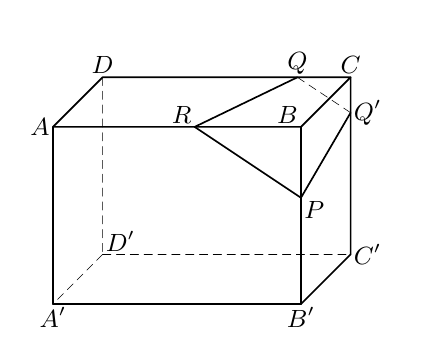
\begin{tikzpicture}[scale=0.45,inner sep=1pt]
  \tkzDefPoints{0/0/A',7/0/B',8.4/1.4/C',1.4/1.4/D',0/5/A,4/5/R,7/3/P,8.4/5.4/Q'}
  \tkzDefPointsBy[translation=from A' to A](B',C',D'){B,C,D}
  \tkzInterLL(B,C)(P,Q')\tkzGetPoint{M}
  \tkzInterLL(M,R)(C,D)\tkzGetPoint{Q}
  \tkzDrawPolygon[semithick](A,B,C,D)
  \tkzDrawSegments[semithick](A,A' A',B' B',C' B',B C',C R,P P,Q' R,Q)
  \tkzDrawSegments[densely dashed](D,D' D',A' D',C' Q,Q')
  \tkzLabelPoints(A',B')
  \tkzLabelPoints[above left](B,R)
  \tkzLabelPoints[above right](D')
  \tkzLabelPoints[below right](P)
  \tkzLabelPoints[left](A)
  \tkzLabelPoints[right](C',Q')
  \tkzLabelPoints[above](C,D,Q)
\end{tikzpicture}
\end{document}